En este capítulo se explica el porqué se han tomado ciertas decisiones, problemas y dudas que han ido surgiendo a lo largo del desarrollo y se muestra las especificaciones del sistema.

\section{Consideraciones de Diseño}
Cuando se utiliza GitHub en el ámbito académico no hay una sola forma de organizar las clases y queda a criterio de cada profesor. Es por esto que una aplicación \emph{opinionated} o inflexible no puede llegar muy lejos. Como resultado, se ha decidido crear un sistema modulable y extendible a través de extensiones, con la aplicación principal manejando información que pueda resultar útil para cualquier extensión futura, pero que sea lo más genérica posible. Esta plasticidad se intenta conseguir mediante la configuración y las extensiones. Por eso se permite en un buen número de puntos  de la configuración , la existencia de campos vacíos y que algunos de estos sean expresiones regulares. De esta forma, diferentes extensiones, pueden utilizar diferentes estrategias y utilizar los datos disponibles como se crea conveniente, haciendo que cada profesor pueda utilizar el programa sin que su metodología de trabajo se vea condicionada.

También tenemos que tener en cuenta que nuestro público objetivo son profesores y alumnos de ingeniería, programación, estadística y relacionados, que utilizan GitHub y que, por lo tanto, tendrán cierto grado de conocimiento con las tecnologías informáticas y la terminal. A su vez, no todas las aplicaciones se van a ver beneficiadas de tener una interfaz gráfica en el navegador y queremos complementar a \verb|GitHub Classroom|, no sustituirlo, por lo que construir el ecosistema en la terminal es la mejor opción.

Las extensiones se subirán a la plataforma de GitHub con el prefijo \verb|gh-edu-|. Se ha elegido tener un \gls{namespace} o prefijo, para diferenciar las extensiones de aquellas extensiones de \verb|gh| que no estén creadas con fines docentes o no tengan intención de aprovecharse del ecosistema.

En un intento de mantener que el ecosistema no sea más complicado de lo necesario, especialmente la interfaz, las peticiones a la \verb|API| de GitHub solo funcionaran con la rama por defecto.

\section{El Núcleo de {\tt gh-edu}}
Construir sobre \verb|gh extension| comandos homónimos como \verb|install| o \verb|remove|, ha sido importante para evitar la reimplementación de un gestor de extensiones desde cero, lo cual hubiese sido excesivo cuando solo se busca tener un mayor control sobre el estado del sistema. También gracias a esto, los creadores de extensiones pueden crear las extensiones en el lenguaje que crean convenientes. Si se trata de un lenguaje interpretado, será suficiente con tener un script escrito en \verb|bash| con el mismo nombre que el del repositorio de GitHub, que se encargue de ejecutar el fichero principal. Para lenguajes compilados es necesario subir los binarios correspondientes al apartado de \verb|Releases| del repositorio y el comando \verb|gh extension install| que se ejecuta internamente se encargará de descargarlo.

\begin{figure}[H]
    \centering
    \makebox[\textwidth][c]{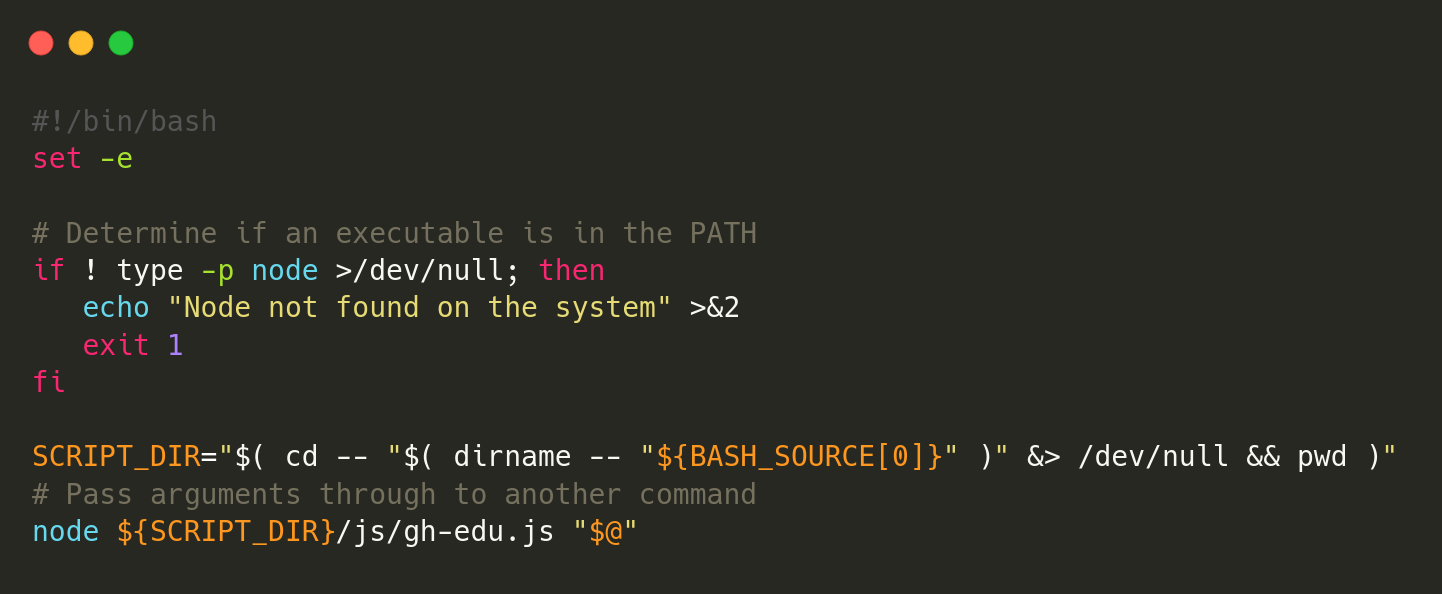
\includegraphics[width=\textwidth]{images/bash.png}}
    \caption{Diseño. Ejemplo de un script para ejecutar una extensión creada con lenguaje interpretado}
    \label{fig:bash}
\end{figure}

\begin{figure}[H]
    \centering
    \makebox[\textwidth][c]{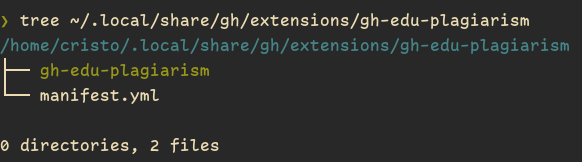
\includegraphics[width=\textwidth]{images/binary.png}}
    \caption{Diseño. Ejemplo de contenido de una extensión creada con lenguaje compilado}
    \label{fig:binario}
\end{figure}

\subsection{El fichero de Configuración {\tt data.json}} \label{diseño:data}

\begin{figure}[H]
    \centering
    \makebox[\textwidth][c]{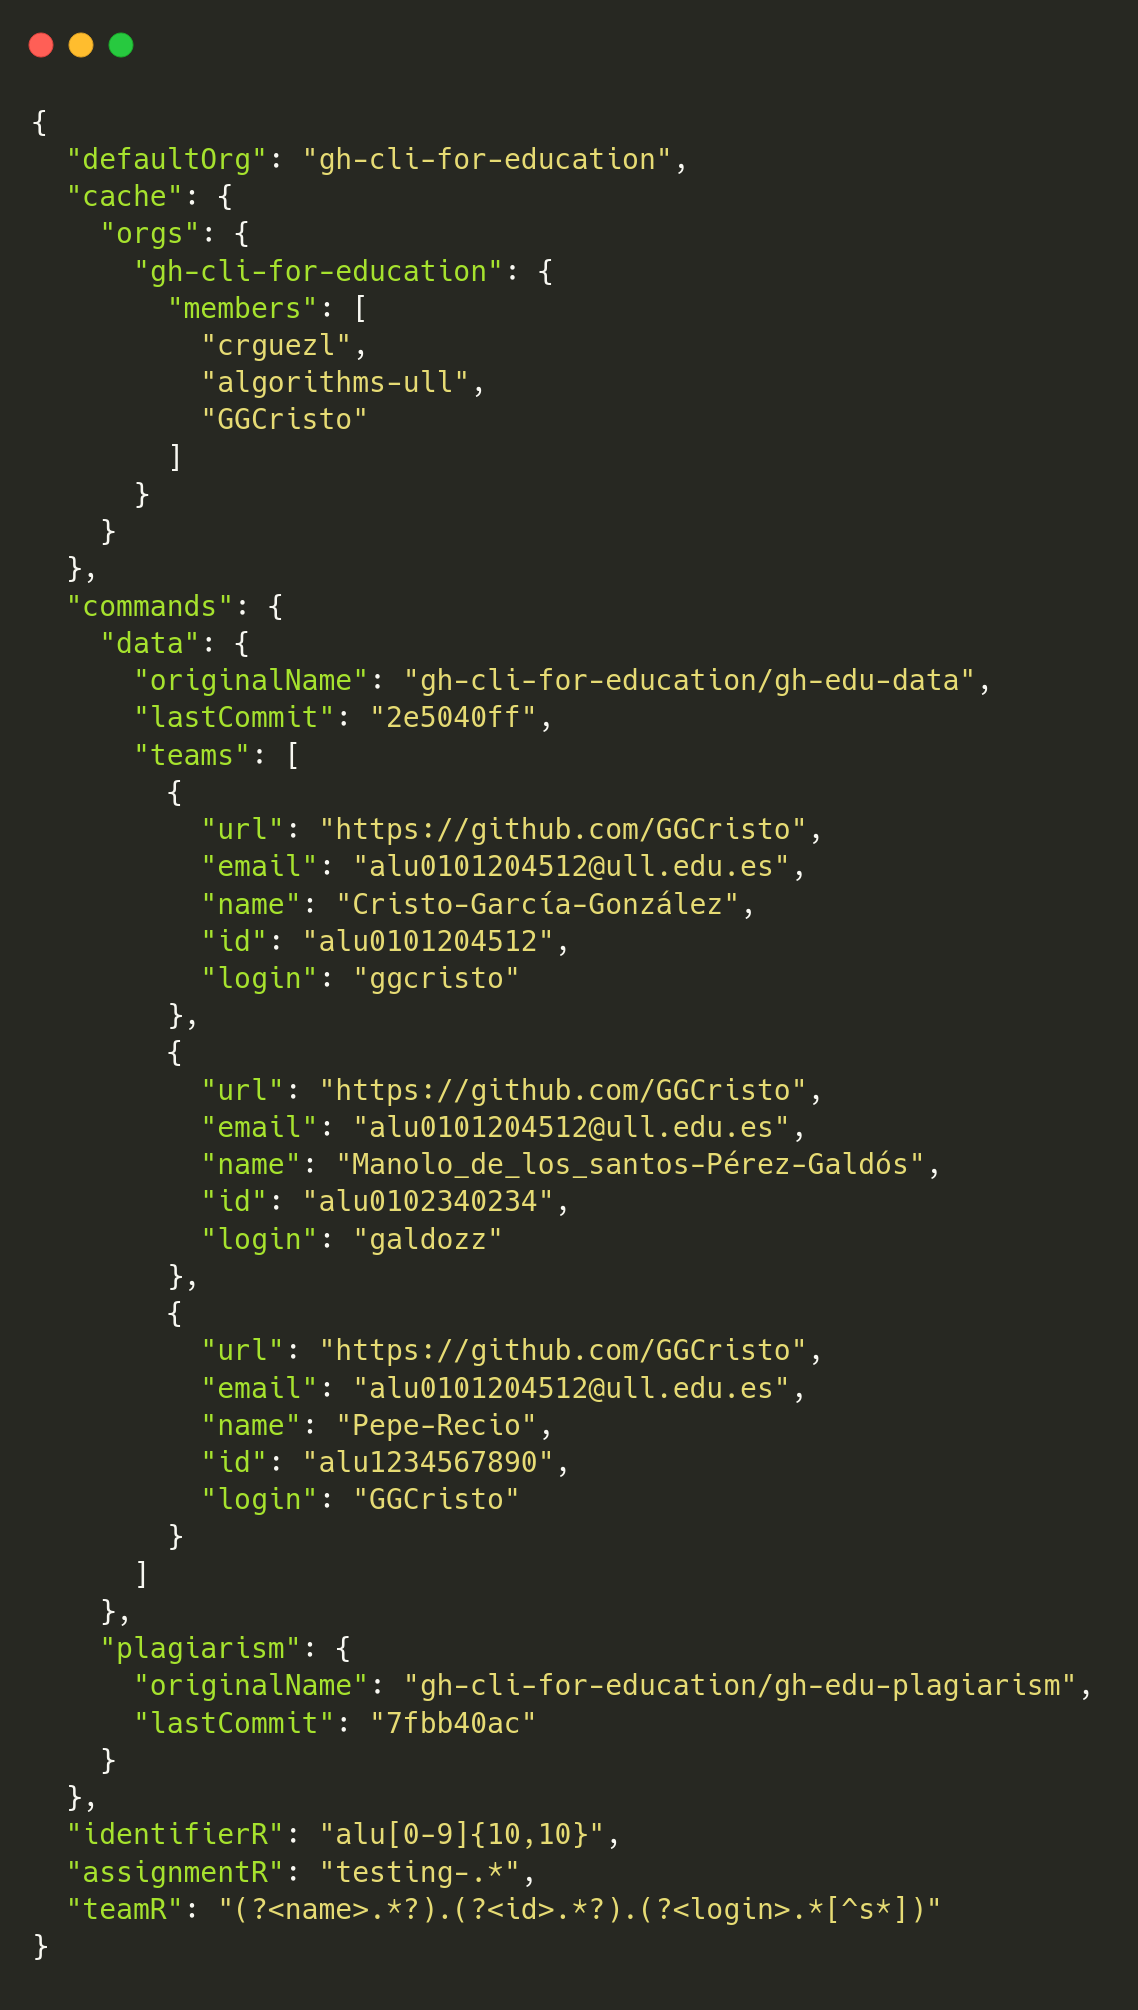
\includegraphics[height=0.5\paperheight]{images/data.png}}
    \caption{Ejemplo de data.json. El comando data tiene su propio campo: teams}
    \label{fig:data}
\end{figure}

El fichero \verb|data.json| es bastante importante. Se trata de un único fichero que actúa como memoria compartida para el intercambio de información entre el usuario, el core y las extensiones. Las extensiones no deben realizar operaciones de lectura, a excepción de una parte dedicada que tiene cada una para guardar sus propios datos (véase \ref{fig:data}). Cabe recordar que este fichero está ubicado en \verb|~/.config/gh-edu/data.json| en sistemas Unix y siempre está bajo gestión de versiones con \verb|Git|.

Tener todos los datos y configuraciones en un único fichero trae la ventaja de la portabilidad. Los usuarios pueden tener un repositorio privado con el nombre de \verb|gh-edu-profile| y así tener siempre una copia asegurada que puede utilizarse en diferentes máquinas.

El esquema mínimo necesario ya se pudo ver en la figura \ref{fig:configType}

\subsection{Integridad de los Datos}

Una extensión maliciosa o mal implementada podría corromper el fichero \verb|data.json|, afectando a otras extensiones. Al tratarse de un fichero, cualquier agente externo ya podía corromperlo, pero la probabilidad de que ocurra aumenta con el número y la calidad de las extensiones. Para intentar paliar esta posibilidad, siempre que se ejecute cualquier comando, el núcleo comprueba que \verb|data.json| es un fichero \verb|JSON| válido y la validez de sus campos (véase \ref{impl:gh-edu-data}). También en caso de error, si el error está relacionado por un campo incorrecto, como tener registrado una organización que no existe o a la cual no se pertenece, se muestra por pantalla el campo incorrecto que provocó el fallo. Junto al apoyo dado por el sistema de versiones, se espera que estas medidas sean suficientes para mejorar la robustez del sistema.


\subsection{Control del Versionado del Sistema}

Otra duda que surge de cara al futuro es como se va a controlar la evolución del controlador, de  \verb|data.json| y como las extensiones deberían reaccionar a dichos cambios. 
El problema surge cuando se introducen cambios en el controlador y el fichero \verb|data.json| que son incompatibles con el pasado. En tal caso el número de major de la versión  del controlador debería haberse incrementado.
Puede ocurrir entonces que una versión de una extensión/plugin de \verb|gh-edu| que funcionaba con una versión anterior del  controlador, deje de funcionar. 

El simple uso del \href{https://semver.org/lang/es/}{versionado semántico}, no resuelve el problema debido a la  posibilidad de un conflicto de dependencias en el que una extensión depende de una versión de \verb|data.json| en específico y otra extensión depende de una diferente. Normalmente con el versionado semántico se tienen las diferentes versiones necesarias de un mismo software, pero esa solución va en contra de la especificación de tener un único fichero. 


Obsérvese que el fichero \verb|data.json| contiene el número de versión semántica del controlador actual:

\begin{verbatim}
                    $ jq '.version' ~/.config/gh-edu/data.json 
                    "0.7.0"
\end{verbatim}

y que dicho número de versión puede ser consultado por cualesquiera extensiones para determinar su compatibilidad con el núcleo/{\emph core}.


En general se intentará mantener la retro-compatibilidad una vez el sistema alcance la estabilidad. Se romperá dicha compatibilidad únicamente en el caso de que sea estrictamente necesario para solucionar un error, notificando de esto a los desarrolladores de extensiones. El fichero \verb|data.json| se mantiene en un repositorio aparte bajo control de versiones. Esta característica debería facilitar la recuperación del sistema en caso de corrupción del fichero o error.


\subsection{El Manejo de la Localidad de los Datos: {\tt cache}}
Algunos comandos pueden llevar tiempo en ejecutarse, especialmente en organizaciones grandes. Es por eso que cierta información se guarda en la entrada \verb|cache| del fichero \verb|data.json| (véase  figura \ref{fig:configType}) y solo se busca y actualiza usando las \verb|API|s cuando la caché no tenga la información necesaria o el usuario desea actualizarla, lo que hará con el comando \verb|gh edu update -c|. 

La caché es un mecanismo de optimización algo peligroso si no se trata con cuidado, es por eso que las extensiones no deberían de escribir en ella. Las extensiones pueden implementar su propia caché en su propia zona asignada. Cabe mencionar que no todos los datos se almacenan en la caché, de momento solo los nombres de las organizaciones y los miembros pertenecientes a ellas son guardados. Se ha elegido estos datos y no otros porque muy rara vez una organización se elimina o renombra y lo mismo pasa con los alumnos o miembros de la organización.

\section{La Extensión gh-edu-plagiarism}
La extensión \verb|plagiarism| fue creada debido a que es uno de los tipos de extensión que más solicitan los profesores en el foro GitHub Classroom Community.

Se ha diseñado para que sea intuitivo y se puede usar tanto de forma interactiva como en un script, utilizando \verb|fzf| solo cuando los datos pasados por parámetros no son suficientes.

El servicio esencial de \verb|plagiarism| es \verb|MOSS|(Measure Of Software Similarity)\cite{MOSS} creado y ubicado en la universidad de Stanford. Se trata de un servicio que recibe código (en ficheros o directorios) y nos devuelve un enlace con un informe por cada combinación de pares posible. 
\begin{figure}
    \centering
    \makebox[\textwidth][c]{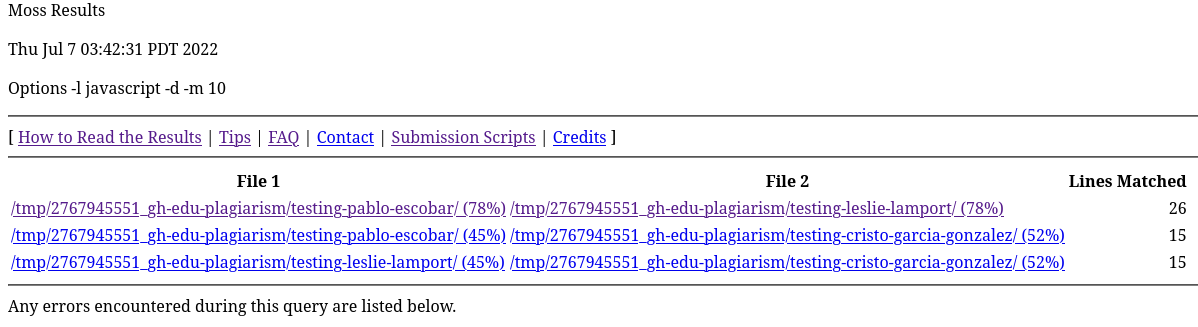
\includegraphics[width=\textwidth]{images/MOSS-raw.png}}
    \caption{Resultado de MOSS sin procesar}
    \label{fig:MOSSRaw}
\end{figure}

\verb|MOSS| es un servicio relativamente popular que lleva usándose desde 1994. Se eligió \verb|MOSS| por encima de otras tecnologías por varios motivos:
\begin{enumerate}
    \item \textbf{Compara cada tarea con el resto de tareas subidas.} Las alternativas comparan el código con código subido en internet. Algunos profesores no consideran plagio que ciertos fragmentos de código estén sacados de internet, incluso se llega a valorar positivamente.
    \item \textbf{Utiliza un algoritmo simple.} Que el algoritmo sea relativamente simple trae muchas ventajas. Por un lado, la ejecución es rápida, algo importante si tenemos en cuenta que se tiene que realizar \(\frac{n!}{(n-2)!2!}\) análisis. Por otro lado, los creadores afirman que después de años de servicio no se les ha informado de falsos positivos\cite{paper} (apartado 5.2 \verb|Plagiarism detection|).
    
    Un algoritmo simple también es suficiente para detectar técnicas comunes realizadas por los alumnos que se copian, como cambiar de nombre las variables, poner espacios en blanco o mover bloques de código de su posición original.
    Esta extensión fue creada para ayudar al profesor a concluir quien puede estar copiándose. No se debe confiar ciegamente en sus resultados.
\end{enumerate}

Otra dependencia menos importante es \verb|mossum|\cite{mossum}, un script hecho en \verb|python| que tiene como input \emph{n} links generados por \verb|MOSS| y que genera un grafo con los porcentajes de similitud entre las asignaciones.

La figura \ref{fig:plagiarism} muestra un diagrama de como funciona la extensión. Ha sido simplificado, ya que el código también se encarga de comprobar que se cumple con los requisitos, hace una configuración inicial y de forma paralela se comprueba en todo momento si ha ocurrido un error y se controla apropiadamente. Esto se conoce como \gls{graceful degradation} y específicamente intenta mostrar algún resultado, incluso si otro falla, en específico si no consigue devolver el informe ni el grafo, retornará un enlace, con una lista de reportes sin procesar, los mismos que devuelve el servidor de \verb|MOSS| (figura \ref{fig:MOSSRaw}).

\begin{figure}[H]
    \centering
    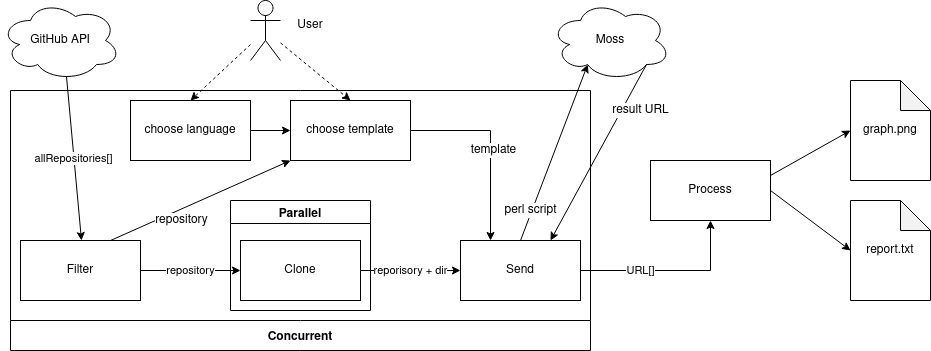
\includegraphics[width=\linewidth]{images/plagiarism.png}
    \caption{Diagrama de funcionamiento de plagiarism}
    \label{fig:plagiarism}
\end{figure}

Entrando en detalle, la aplicación 
\begin{enumerate}
    \item \textbf{GitHub API.} Empieza pidiendo todos los repositorios de la organización.
    \item \textbf{Filter.} Después pasa por un filtrado para quedarse con los repositorios que si interesan que sería aquellos relacionados con la tarea actual de la asignatura, utilizando expresiones regulares.
    \item \textbf{Clone.} Los repositorios se van clonando en paralelo en un directorio temporal del sistema.
    \item \textbf{Send.} A medida que se van clonando se les adjunta la dirección absoluta y se va preparando para ser enviados al servidor de \verb|MOSS| a través de su script.
    \item \textbf{Process.} Una vez \verb|MOSS| haya devuelto el enlace con los informes. ejecutamos el programa \verb|mossum| para la generación del grafo y la obtención del informe separado por pares de alumnos. Cuando el programa termina se muestra por pantalla un informe de todos los pares para que el profesor pueda ver las diferencias y determinar si de verdad hubo plagio (figura \ref{fig:reportPlagiarism}) y el susodicho grafo (figura \ref{fig:graphMossum}).
\end{enumerate}

Desde que el programa empieza se le pide al usuario información necesaria, en el caso de que no lo haya especificado por línea de comandos, como puede ser 
\begin{itemize}
    \item el lenguaje de programación utilizado en el código o
    \item una plantilla que el profesor haya proporcionado a los alumnos y sirva de base (en caso de haberla)
\end{itemize}

\begin{figure}[H]
    \centering
    \makebox[\textwidth][c]{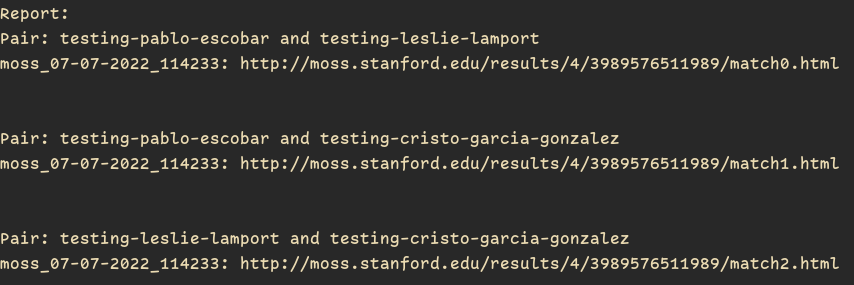
\includegraphics[width=\textwidth]{images/report-plagiarism.png}}
    \caption{Informe final dado por plagiarsim, con enlace para comprobar el código manualmente}
    \label{fig:reportPlagiarism}
\end{figure}

\begin{figure}[H]
    \centering
    \makebox[\textwidth][c]{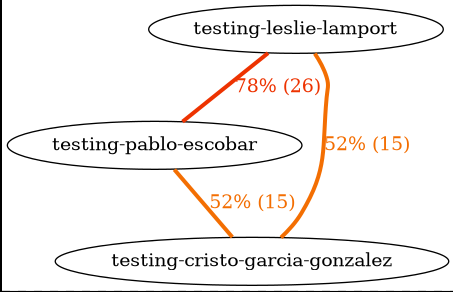
\includegraphics[width=0.5\textwidth]{images/grafo-moss.png}}
    \caption{Plagiarism. Grafo resultante mostrando los niveles de similitud}
    \label{fig:graphMossum}
\end{figure}

\emph{Nota: Debido a la política de privacidad de MOSS los informes pueden estar disponibles por 14 días, aunque también se avisa que existe la posibilidad de que se eliminen antes para poder liberar memoria de los servidores si se alcanza cierto límite no estipulado.}

La extensión \verb|plagiarism| funciona bastante bien con el sistema \verb|gh-edu|, pero también se ha diseñado para que sea posible su uso de forma independiente.
